\documentclass[a4paper]{article}
\usepackage{times}
\usepackage[utf8]{inputenc}
\usepackage[T1]{fontenc}
\usepackage{selinput}
\usepackage{upquote}
\usepackage[margin=2cm, rmargin=4cm, tmargin=3cm]{geometry}
\usepackage{tcolorbox}
\usepackage{xspace}
\usepackage{amsmath}
\usepackage{float}
\usepackage[french]{babel}
\usepackage{hyperref}
\usepackage{xurl}
\usepackage{fontawesome6}
\usepackage{enumitem}
\usepackage{marginnote}
\usepackage{ulem}
\usepackage[yyyymmdd,hhmmss]{datetime}
\usepackage{ulem}
\usepackage{environ}
\usepackage{graphicx}
%\usepackage[top=Bcm, bottom=Hcm, outer=Ccm, inner=Acm, heightrounded, marginparwidth=Ecm, marginparsep=Dcm]{geometry}
\usepackage{courier}



\newtcolorbox{Example}[1]{colback=white,left=20pt,colframe=slideblue,fonttitle=\bfseries,title=#1}
\newtcolorbox{Solutions}[1]{colback=white,left=20pt,colframe=green,fonttitle=\bfseries,title=#1}
\newtcolorbox{Conseils}[1]{colback=white,left=20pt,colframe=slideblue,fonttitle=\bfseries,title=#1}
\newtcolorbox{Warning}[1]{colback=white,left=20pt,colframe=warning,fonttitle=\bfseries,title=#1}
\newtcolorbox{Note}[1]{colback=white,left=20pt,colframe=grey,fonttitle=\bfseries,title=#1}
\newtcolorbox{Dessin}[1]{colback=white,left=20pt,colframe=grey,fonttitle=\bfseries,title=#1}

\setlength\parindent{0pt}

  %Exercice environment
  \newcounter{exercice}
  \newenvironment{Exercice}[1][]
  {
  \par
  \stepcounter{exercice}\textbf{Question \arabic{exercice}:} (\faClock \enskip \textit{#1})
  }
  {\bigskip}
  

% Title
\newcommand{\titre}{\begin{center}
  \section*{Algorithmes et Pensée Computationnelle}
\end{center}}
\newcommand{\cours}[1]
{\begin{center} 
  \textit{#1}\\
\end{center}
  }



% \newcommand{\exemple}[1]{\newline~\textbf{Exemple :} #1}
\newcommand{\todo}[1]{\textcolor{red}{#1}}
%\newcommand{\attention}[1]{\newline\faExclamationTriangle~\textbf{Attention :} #1}

% Documentation url (escape \# in the TP document)
\newcommand{\documentation}[1]{\faBookOpen~Documentation : \href{#1}{#1}}

% Clef API
\newcommand{\apikey}[1]{\faKey~Clé API : \lstinline{#1}}
\newcommand{\apiendpoint}[1]{\faGlobe~Url de base de l'API \href{#1}{#1}}

%Listing Python style
\usepackage{color}
\definecolor{slideblue}{RGB}{33,131,189}
\definecolor{green}{RGB}{0,190,100}
\definecolor{blue}{RGB}{121,142,213}
\definecolor{grey}{RGB}{120,120,120}
\definecolor{warning}{RGB}{235,186,1}

\usepackage{listings}
\lstdefinelanguage{texte}{
    keywordstyle=\color{black},
    numbers=none,
    frame=none,
    literate=
           {é}{{\'e}}1
           {è}{{\`e}}1
           {ê}{{\^e}}1
           {à}{{\`a}}1
           {â}{{\^a}}1
           {ù}{{\`u}}1
           {ü}{{\"u}}1
           {î}{{\^i}}1
           {ï}{{\"i}}1
           {ë}{{\"e}}1
           {Ç}{{\,C}}1
           {ç}{{\,c}}1
           {ô}{{\^o}}1,
    columns=fullflexible,keepspaces,
	breaklines=true,
	breakatwhitespace=true,
}
\lstset{
  language=Python,
	%basicstyle=\bfseries\footnotesize,
  basicstyle=\footnotesize\ttfamily\small,
	breaklines=true,
	breakatwhitespace=true,
	commentstyle=\color{grey},
	stringstyle=\color{slideblue},
  keywordstyle=\color{slideblue},
	morekeywords={with, as, True, False, Fraction, Float, join, index, None, main, argparse, self, sort, __eq__, __add__, __mul__ ,__ne__, __radd__, __del__, __ge__, __gt__, split, os, endswith, is_file, scandir, @classmethod, this},
	deletekeywords={id},
	showspaces=false,
	showstringspaces=false,
	columns=fullflexible,keepspaces,
	literate=
           {é}{{\'e}}1
           {è}{{\`e}}1
           {ê}{{\^e}}1
           {à}{{\`a}}1
           {â}{{\^a}}1
           {ù}{{\`u}}1
           {ü}{{\"u}}1
           {î}{{\^i}}1
           {ï}{{\"i}}1
           {ë}{{\"e}}1
           {Ç}{{\,C}}1
           {ç}{{\,c}}1
           {ô}{{\^o}}1,
    numbers=left,
}

\newtcbox{\mybox}{nobeforeafter,colframe=white,colback=slideblue,boxrule=0.5pt,arc=1.5pt, boxsep=0pt,left=2pt,right=2pt,top=2pt,bottom=2pt,tcbox raise base}
\newcommand{\projet}{\mybox{\textcolor{white}{\small projet}}\xspace}
\newcommand{\optionnel}{\mybox{\textcolor{white}{\small Optionnel}}\xspace}
\newcommand{\advanced}{\mybox{\textcolor{white}{\small Pour aller plus loin}}\xspace}
\newcommand{\auto}{\mybox{\textcolor{white}{\small Auto-évaluation}}\xspace}


\usepackage{environ}
\newif\ifShowSolution
\NewEnviron{solution}{
  \ifShowSolution
	\begin{Solutions}{\faTerminal \enskip Solution}
		\BODY
	\end{Solutions}
  \fi}

\usepackage{environ}
\newif\ifShowExample
\NewEnviron{exemple}{
  \ifShowExample
	\begin{Example}{\faTerminal \enskip Exemple}
		\BODY
	\end{Example}
  \fi}

\usepackage{environ}
 \newif\ifShowConseil
  \NewEnviron{conseil}{
    \ifShowConseil
    \begin{Conseils}{\faLightbulb \quad Conseil}
      \BODY
    \end{Conseils}

    \fi}

    \usepackage{environ}
  \newif\ifShowWarning
  \NewEnviron{attention}{
    \ifShowWarning
    \begin{Warning}{\faTriangleExclamation \quad Attention}
      \BODY
    \end{Warning}

    \fi}

  \newif\ifShowNote
  \NewEnviron{note}[1]{
    \ifShowNote
    \begin{Note}{\faEye \quad Comment added by #1 at \date - \currenttime}
      \BODY
    \end{Note}

    \fi}  

    \newif\ifShowDessin
    \NewEnviron{dessin}[1]{
      \ifShowDessin
      \begin{Dessin}{\faPen \quad Figure}
        \BODY
      \end{Dessin}
  
      \fi}  

%\newcommand{\Conseil}[1]{\ifShowIndice\ \newline\faLightbulb[regular]~#1\fi}

\usepackage{tikz}
\usetikzlibrary{arrows.meta}
\graphicspath{{img/}}

% Les flèches utilisent des coordonnées normalisées par rapport aux captures d'écran.
\definecolor{noticearrow}{RGB}{204,72,32}
\tikzset{
  notice arrow/.style={draw=noticearrow, line width=2.2pt, -{Stealth[length=4mm]}},
  notice badge/.style={circle, draw=noticearrow, line width=1pt,
    fill=white, text=noticearrow, font=\bfseries\small,
    inner sep=1pt, minimum size=5.5mm}
}
\newcommand{\stepmark}[5]{%
  \node[notice badge] (step#1) at (#2,#3) {#1};
  \draw[notice arrow] (step#1) -- (#4,#5);
}
\newcommand{\shotcaption}[1]{\par\smallskip{\small\itshape #1}\par\medskip}

\begin{document}
\titre
\cours{Premiers pas avec Python dans IntelliJ IDEA}

La semaine dernière, vous avez appris à créer et à exécuter des programmes depuis la ligne de commande, notamment en leur passant des arguments. Cette semaine, vous allez voir comment réaliser ces mêmes tâches directement dans IntelliJ IDEA.

\section{Créer un projet Python dans IntelliJ IDEA}

Ouvrez IntelliJ IDEA. Sur l'écran d'accueil, sélectionnez \textbf{New Project}.

\begin{center}
\begin{tikzpicture}
  \node[anchor=south west,inner sep=0] (screen) at (0,0)
    {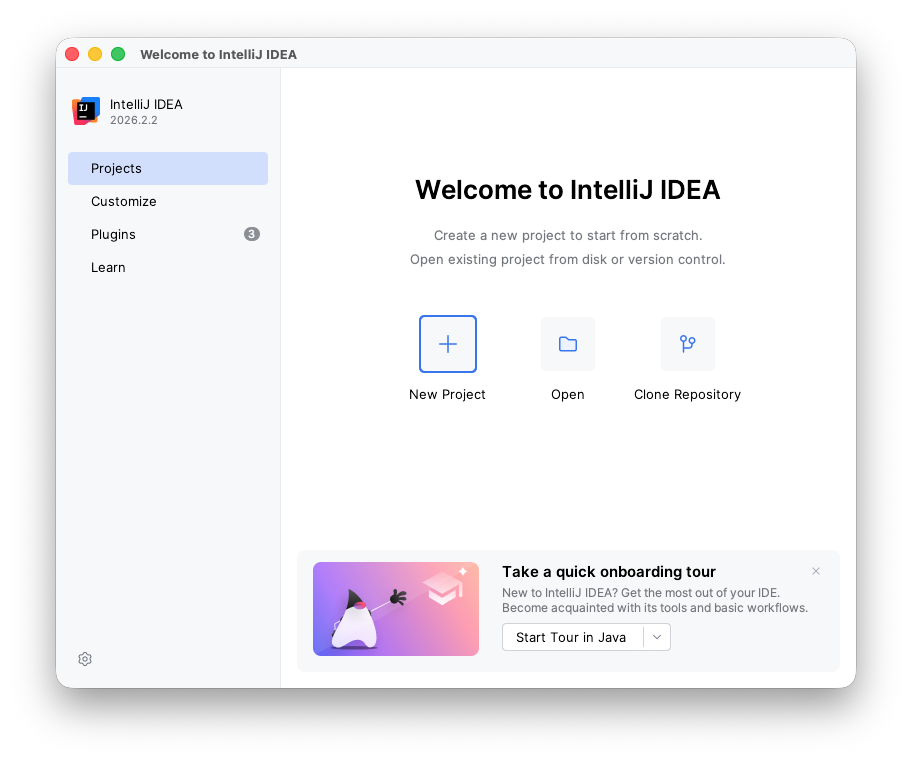
\includegraphics[width=.55\linewidth]{launchIntellij.png}};
  \begin{scope}[x={(screen.south east)},y={(screen.north west)}]
    \stepmark{1}{.72}{.67}{.49}{.55}
  \end{scope}
\end{tikzpicture}
\shotcaption{L'écran d'accueil d'IntelliJ IDEA.}
\end{center}

Dans la fenêtre de création du projet, choisissez \textbf{Python} (1), indiquez
un nom et un emplacement pour le projet (2), puis sélectionnez un interpréteur
Python (3). La capture montre un environnement virtuel propre au projet. Votre
version de Python et vos chemins d'accès peuvent être différents. Sélectionnez
\textbf{Create} (4).

\begin{center}
\begin{tikzpicture}
  \node[anchor=south west,inner sep=0] (screen) at (0,0)
    {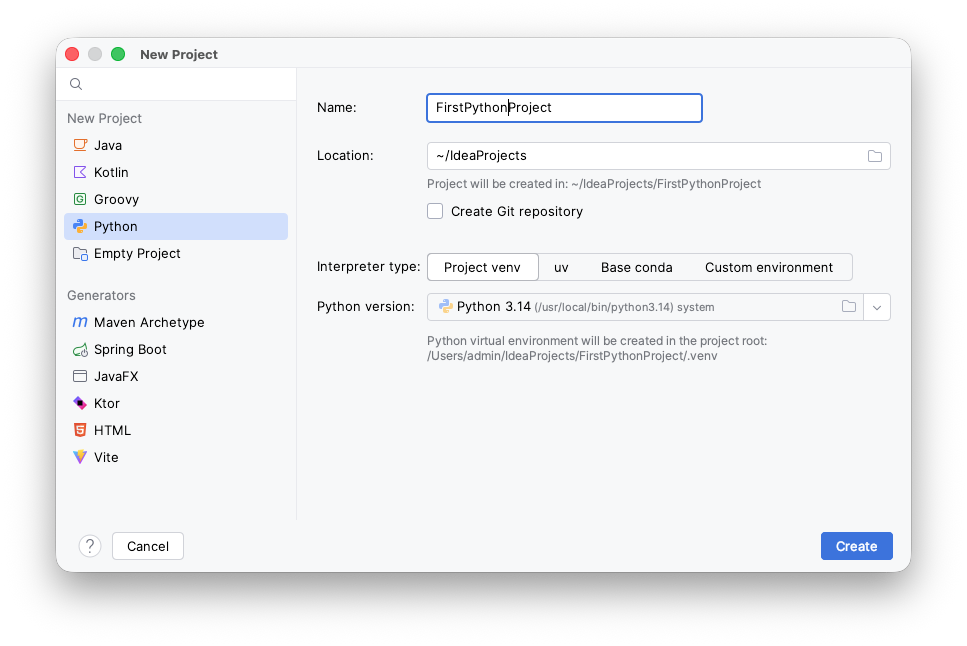
\includegraphics[width=.78\linewidth]{creatingProject.png}};
  \begin{scope}[x={(screen.south east)},y={(screen.north west)}]
    \stepmark{1}{.35}{.73}{.17}{.65}
    \stepmark{2}{.70}{.89}{.56}{.83}
    \stepmark{3}{.75}{.58}{.55}{.52}
    \stepmark{4}{.71}{.16}{.88}{.15}
  \end{scope}
\end{tikzpicture}
\shotcaption{Choisissez Python, nommez le projet, vérifiez l'interpréteur et créez le projet.}
\end{center}

\clearpage
\subsection*{Créer un fichier Python}

Dans le panneau \textbf{Project}, faites un clic droit sur le nom du projet (1),
choisissez \textbf{New} (2), puis \textbf{Python File} (3). Les deux menus
ci-dessous se superposent à la fenêtre du projet, comme dans IntelliJ IDEA.

\begin{center}
\begin{tikzpicture}
  \node[anchor=south west,inner sep=0] (screen) at (0,0)
    {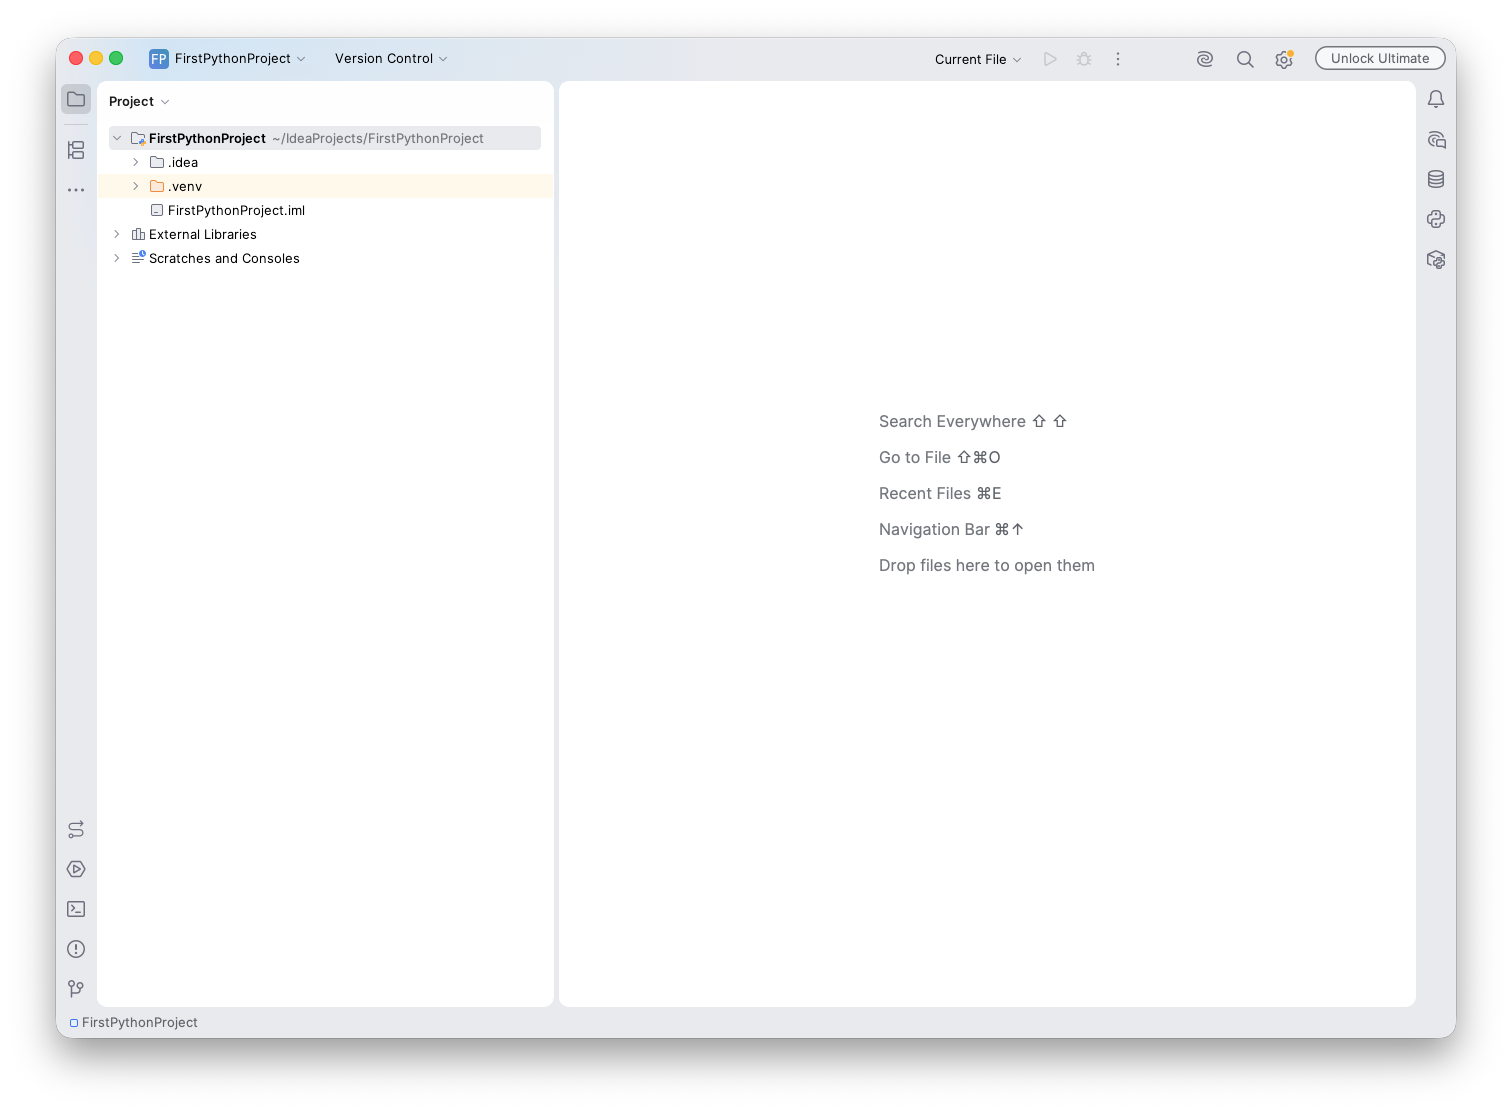
\includegraphics[width=\linewidth]{leftmostSubwindow.png}};
  \begin{scope}[x={(screen.south east)},y={(screen.north west)}]
    % Conserver l'échelle relative des captures recadrées des menus.
    % Le menu de droite recouvre légèrement le bord du premier menu.
    \node[anchor=north west,inner sep=0] at (.17,0.88)
      {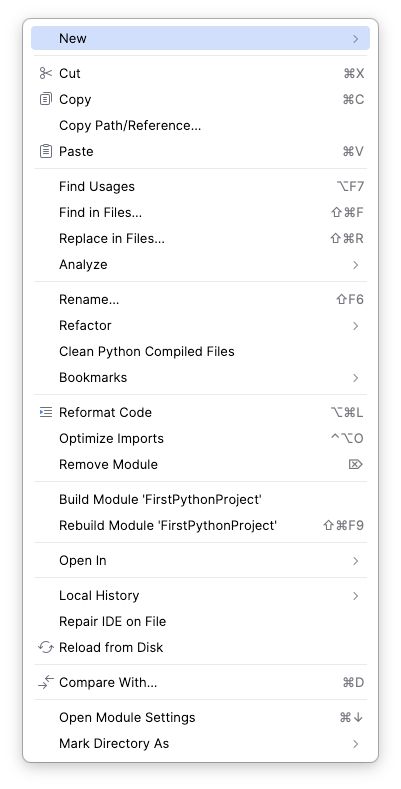
\includegraphics[width=.265\linewidth]{middleSubwindow.png}};
    \node[anchor=north west,inner sep=0] at (.41,.875)
      {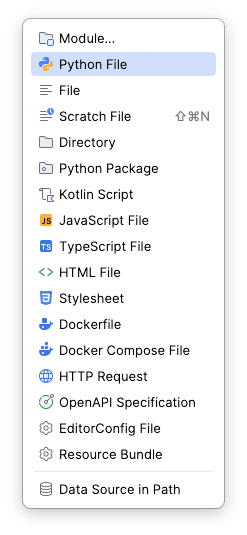
\includegraphics[width=.163\linewidth]{rightmostSubwindow.png}};
    \stepmark{1}{.08}{.92}{.16}{.88}
    \stepmark{2}{.35}{.94}{.23}{.86}
    \stepmark{3}{.69}{.89}{.5}{.81}
  \end{scope}
\end{tikzpicture}
\shotcaption{La fenêtre du projet et les deux menus contextuels dans leur ordre d'apparition.}
\end{center}

Saisissez \lstinline{main} comme nom de fichier, laissez \textbf{Python file}
sélectionné, puis appuyez sur Entrée. IntelliJ ajoute l'extension
\lstinline{.py}.

\begin{center}
\begin{tikzpicture}
  \node[anchor=south west,inner sep=0] (screen) at (0,0)
    {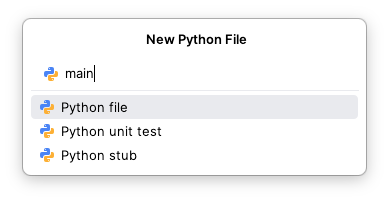
\includegraphics[width=.60\linewidth]{specifyFileName.png}};
  \begin{scope}[x={(screen.south east)},y={(screen.north west)}]
    \stepmark{1}{.77}{.72}{.22}{.63}
  \end{scope}
\end{tikzpicture}
\shotcaption{Nommez le nouveau fichier main.py.}
\end{center}

\clearpage
Le fichier apparaît maintenant dans le panneau \textbf{Project} (1), et son
éditeur vide s'ouvre à droite (2). Cliquez dans l'éditeur pour saisir du code
Python.

\begin{center}
\begin{tikzpicture}
  \node[anchor=south west,inner sep=0] (screen) at (0,0)
    {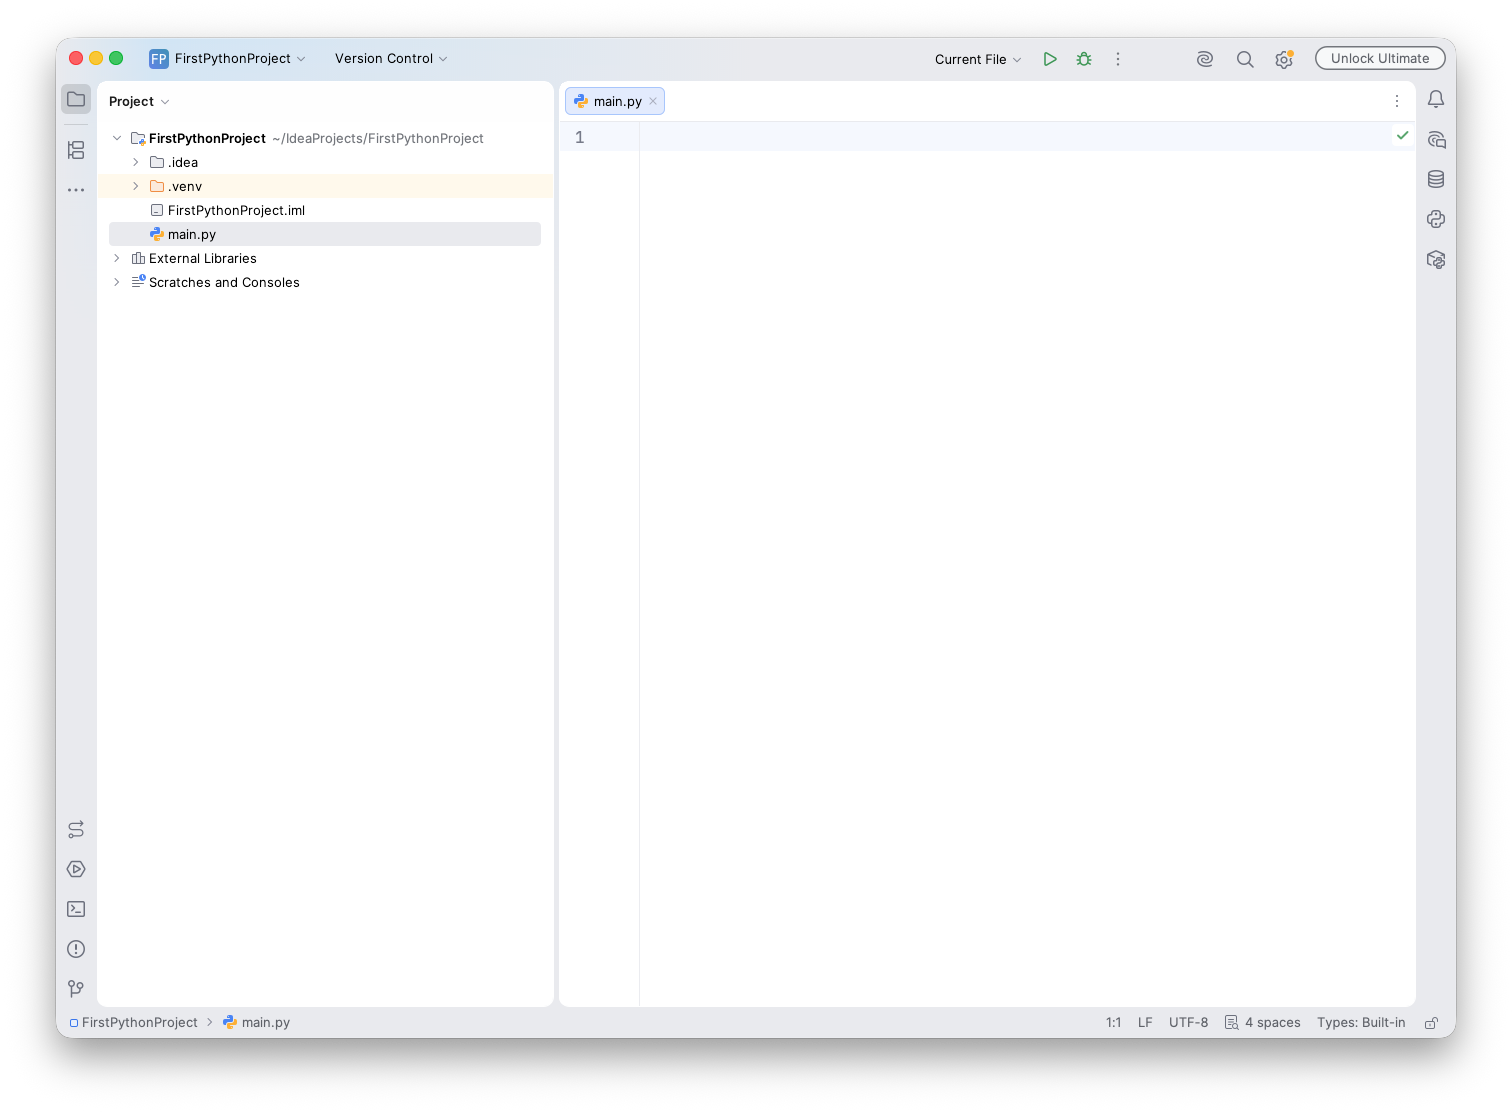
\includegraphics[width=.65\linewidth]{emptyEditor.png}};
  \begin{scope}[x={(screen.south east)},y={(screen.north west)}]
    \stepmark{1}{.31}{.87}{.13}{.79}
    \stepmark{2}{.76}{.80}{.48}{.87}
  \end{scope}
\end{tikzpicture}
\shotcaption{Le nouveau fichier dans le panneau du projet et sa zone d'édition.}
\end{center}

\section{Créer des variables}

Une variable associe un nom à une valeur. En Python, on attribue une valeur
avec \lstinline{=} : \lstinline{a = 1} stocke un nombre, \lstinline{b = "beta"}
stocke du texte et \lstinline{c = False} stocke une valeur booléenne. Il n'est
pas nécessaire de déclarer le type à l'avance. Dans la capture,
\lstinline{d = a} copie la valeur actuelle de \lstinline{a}. Après
\lstinline{a = 2}, \lstinline{d} vaut toujours \lstinline{1}. Les deux lignes
du panneau \textbf{Run} montrent cette différence.

\begin{center}
\begin{tikzpicture}
  \node[anchor=south west,inner sep=0] (screen) at (0,0)
    {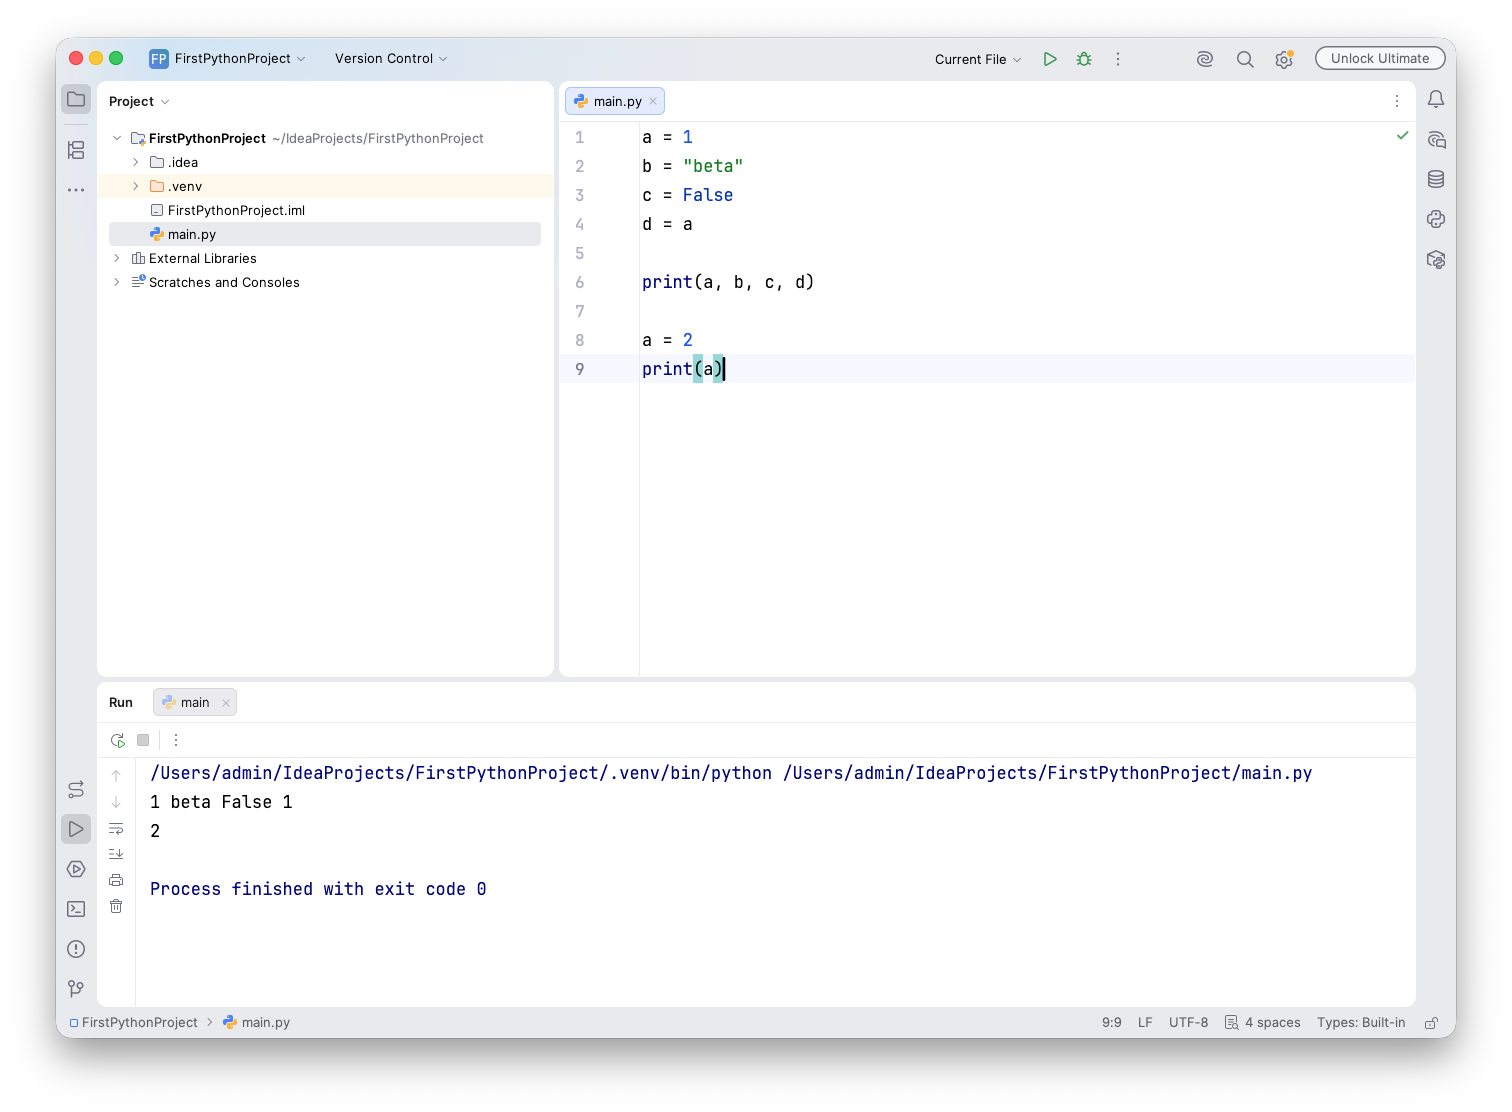
\includegraphics[width=.92\linewidth]{creatingVariables.png}};
  \begin{scope}[x={(screen.south east)},y={(screen.north west)}]
    \stepmark{1}{.75}{.80}{.47}{.875}
    \stepmark{2}{.74}{.67}{.47}{.695}
    \stepmark{3}{.55}{.32}{.12}{.255}
  \end{scope}
\end{tikzpicture}
\shotcaption{Les affectations (1), la réaffectation (2) et les résultats affichés (3).}
\end{center}

\clearpage
\section{L'importance de l'indentation}

En Python, l'indentation regroupe les instructions en blocs. Une ligne terminée
par deux-points, comme la ligne \lstinline{if} ci-dessous, doit être suivie
d'un bloc indenté. Dans la première capture, \lstinline{a = 2} reste aligné
sur la marge gauche : Python signale donc une erreur
\lstinline{IndentationError} (flèche 1).

\begin{center}
\begin{tikzpicture}
  \node[anchor=south west,inner sep=0] (screen) at (0,0)
    {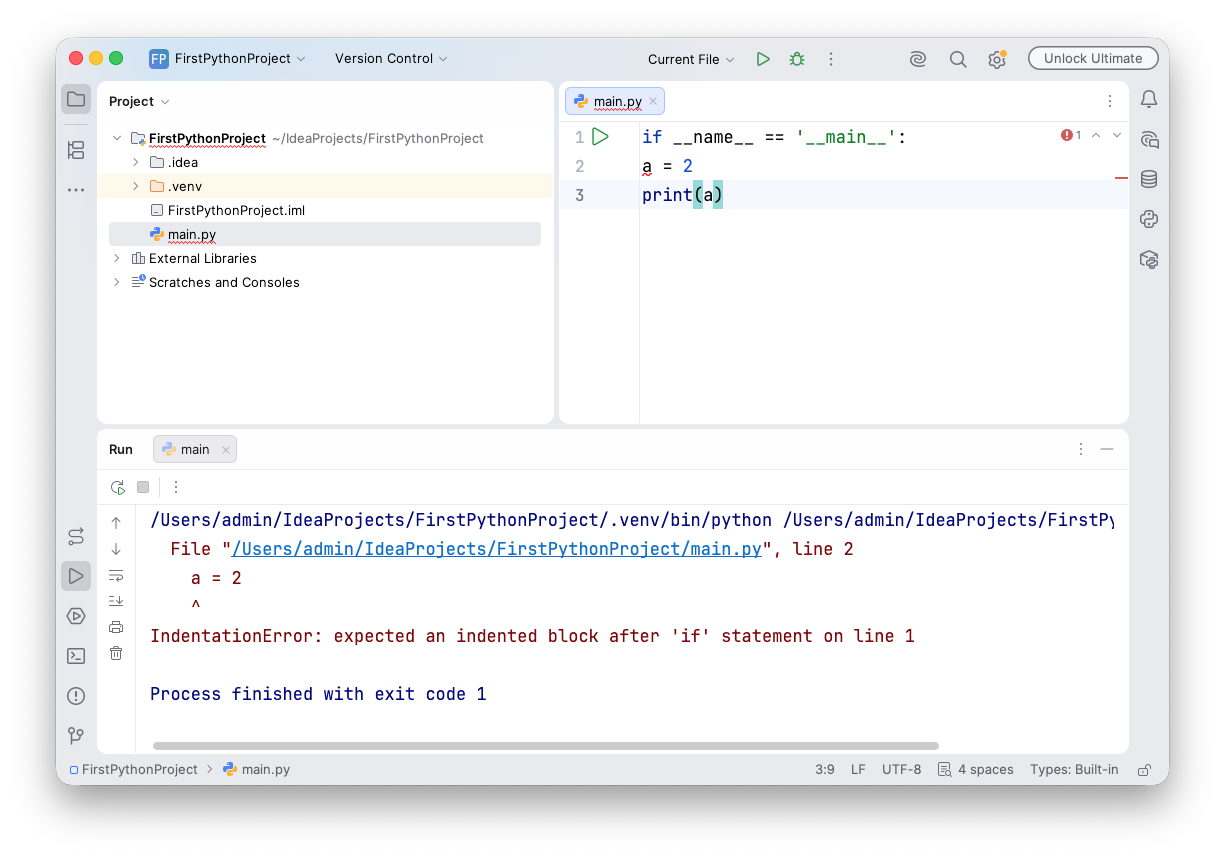
\includegraphics[width=.86\linewidth]{badIndent.png}};
  \begin{scope}[x={(screen.south east)},y={(screen.north west)}]
    \stepmark{1}{.78}{.59}{.44}{.26}
  \end{scope}
\end{tikzpicture}
\shotcaption{Aucun bloc indenté ne suit la condition : le programme s'arrête avec une erreur.}
\end{center}

Indentez les deux instructions sous la ligne \lstinline{if}, comme dans la
version corrigée (flèche 1). Quatre espaces constituent un niveau d'indentation
courant. Le panneau \textbf{Run} affiche maintenant \lstinline{2} (flèche 2).
Les instructions d'un même bloc doivent être alignées au même niveau.

\begin{center}
\begin{tikzpicture}
  \node[anchor=south west,inner sep=0] (screen) at (0,0)
    {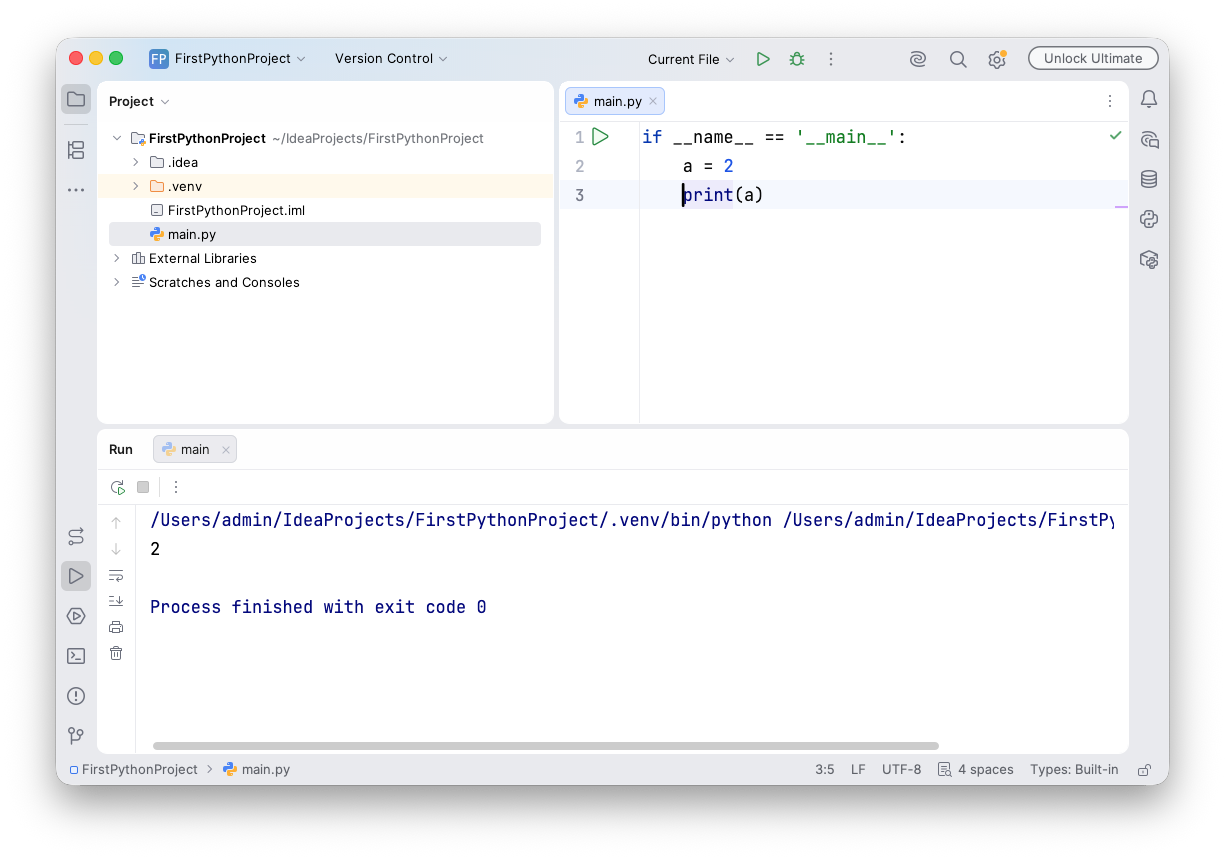
\includegraphics[width=.86\linewidth]{goodIndent.png}};
  \begin{scope}[x={(screen.south east)},y={(screen.north west)}]
    \stepmark{1}{.76}{.33}{.55}{.79}
    \stepmark{2}{.50}{.28}{.13}{.36}
  \end{scope}
\end{tikzpicture}
\shotcaption{Les deux instructions sont indentées : le programme s'exécute et affiche 2.}
\end{center}

\clearpage
\section{Les fonctions}

\lstinline{print()} est une fonction Python. Elle affiche dans le panneau
\textbf{Run} la valeur placée entre ses parenthèses. Saisissez
\lstinline{print("votre message")} (flèche 1), puis cliquez sur le bouton vert
d'exécution en haut de la fenêtre. Le résultat est
\lstinline{votre message} (flèche 2) : les guillemets délimitent le texte
dans le code, mais ne sont pas affichés.

\begin{center}
\begin{tikzpicture}
  \node[anchor=south west,inner sep=0] (screen) at (0,0)
    {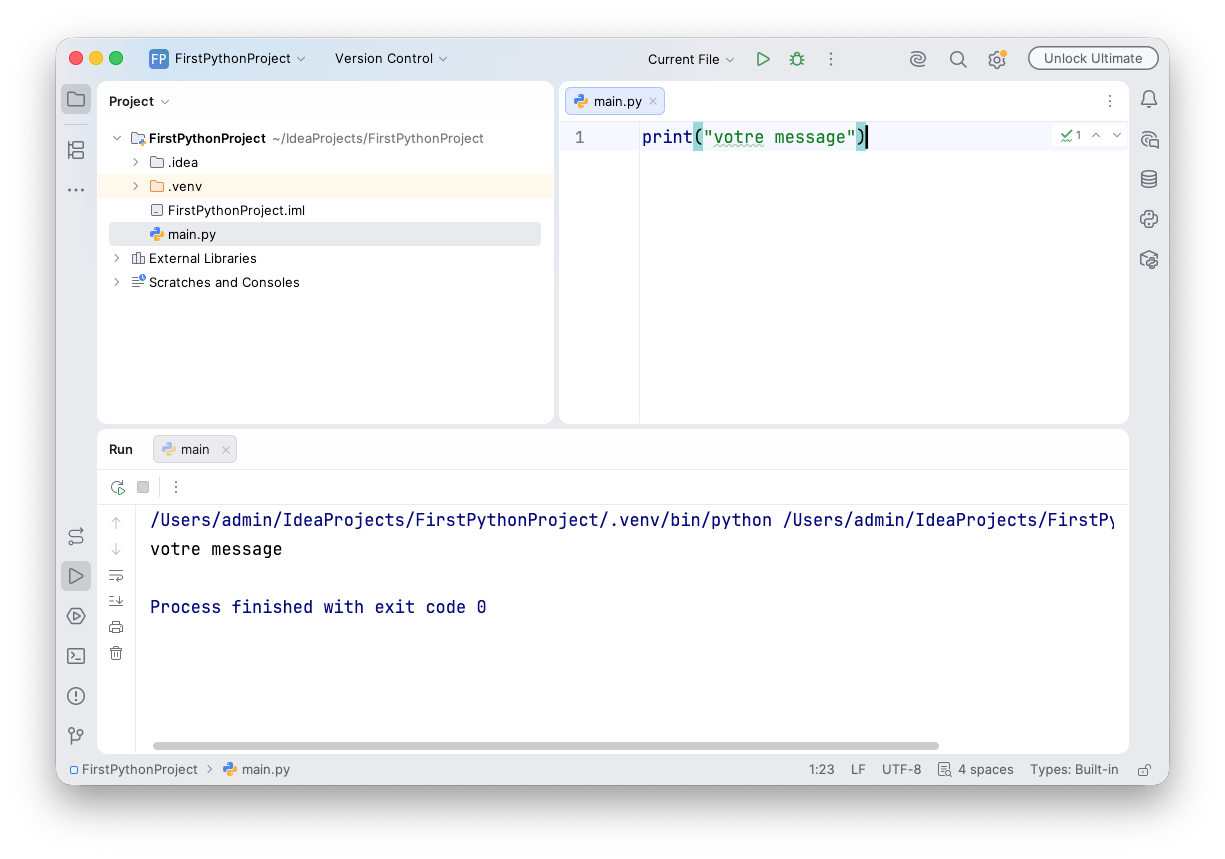
\includegraphics[width=.91\linewidth]{functionExample.png}};
  \begin{scope}[x={(screen.south east)},y={(screen.north west)}]
    \stepmark{1}{.77}{.78}{.60}{.84}
    \stepmark{2}{.52}{.30}{.18}{.36}
  \end{scope}
\end{tikzpicture}
\shotcaption{L'appel de la fonction print() dans l'éditeur et son résultat dans le panneau d'exécution.}
\end{center}

\section{Les arguments de la ligne de commande}

Les arguments de la ligne de commande sont des valeurs transmises au lancement
d'un programme. Dans \lstinline{main.py}, saisissez \lstinline{import sys},
puis \lstinline{print(sys.argv[1])}. Ici, \lstinline{sys.argv[1]} désigne le
premier argument fourni par l'utilisateur ; \lstinline{sys.argv[0]} contient
le nom du programme. Ouvrez le menu à trois points à côté des commandes
d'exécution, puis choisissez \textbf{Run with Parameters...} (flèche 1).

\begin{center}
\begin{tikzpicture}
  \node[anchor=south west,inner sep=0] (screen) at (0,0)
    {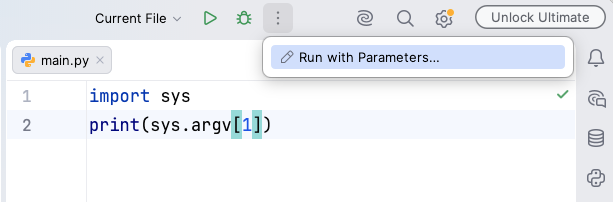
\includegraphics[width=.84\linewidth]{runWithParameters.png}};
  \begin{scope}[x={(screen.south east)},y={(screen.north west)}]
    \stepmark{1}{.75}{.22}{.67}{.72}
  \end{scope}
\end{tikzpicture}
\shotcaption{La commande de lancement avec paramètres et le programme qui lit un argument.}
\end{center}

\clearpage
Dans \textbf{Script parameters}, saisissez
\lstinline{firstParam SecondParam} (flèche 1), puis sélectionnez
\textbf{Run} (flèche 2). IntelliJ transmet les deux mots comme deux arguments
distincts. Le programme affiche \lstinline{firstParam}, car il utilise
\lstinline{sys.argv[1]} ; \lstinline{sys.argv[2]} désignerait
\lstinline{SecondParam}. Fournissez au moins un argument avant d'exécuter
ce programme.

\begin{center}
\begin{tikzpicture}
  \node[anchor=south west,inner sep=0] (screen) at (0,0)
    {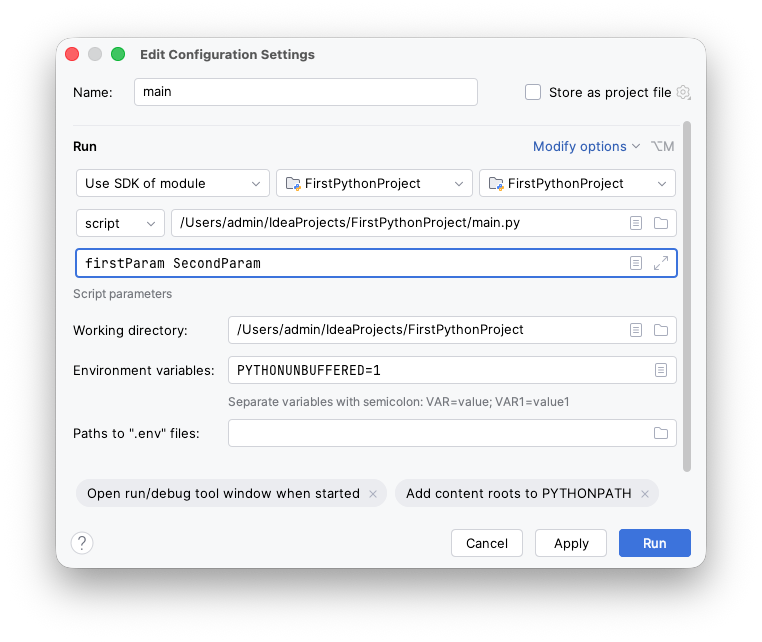
\includegraphics[width=.84\linewidth]{specifyParameters.png}};
  \begin{scope}[x={(screen.south east)},y={(screen.north west)}]
    \stepmark{1}{.77}{.76}{.43}{.59}
    \stepmark{2}{.66}{.20}{.86}{.15}
  \end{scope}
\end{tikzpicture}
\shotcaption{Saisissez les paramètres du programme, puis lancez son exécution.}
\end{center}

\end{document}
